\chapter{Zadanie 3}
\thispagestyle{chapterBeginStyle}
\label{rozdzial3}
\section{Opis problemu}
Zadanie polega na rozwiązaniu problemu minimalizacji kosztu pewnej rafinerii dysponującą jednostką destylacji
(pozwalającą otrzymywać cztery rodzaje produktów: poliwa silnikowe, oleje, destylaty ciężkie i resztki),
jednostką reformowania oraz jednostką krakowania katalitycznego (która może przetwarzać destylaty ciężkie). 
Cały proces przedstawiony jest na rysuku \ref{rafineria}. Celem tego zadania, jest znalezienie odpowiedzi na pytania: 

\begin{itemize}
    \item ile ropy danego rodzaju należy kupić;
    \item jaką część półproduktów przeznaczyć do produkcji poszczególnych produktów;
    \item jaką część półproduktów przeznaczyć do jednostki krakowania katalitycznego.
\end{itemize}

\begin{figure}[h]
    \centering
    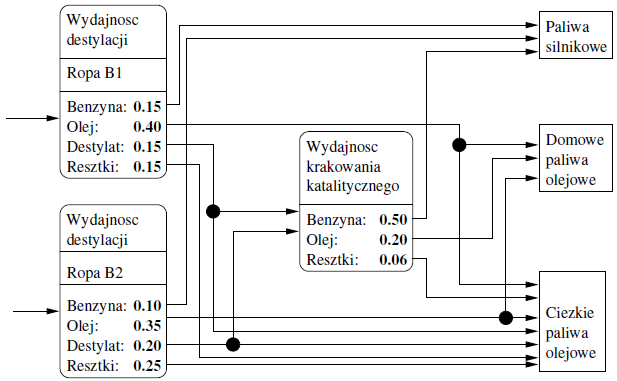
\includegraphics[scale=0.95]{zad3.png}
    \caption{Schemat destylacji}
    \label{rafineria}
\end{figure}
\ \\
\section{Opis problemu}
Do rozwiązania problemu stworzono model z parametrami: 
\begin{itemize}
    \item $KoszRopy_{r}$ gdzie $r \in RodzajRopy$ koszt danego rodzaju ropy;
    \item $KosztReformowania$ koszt destylacji ropy każdego rodzaju;
    \item $KosztKrakowania$ koszt krakowania pół produktów każdego typu;
    \item $WydajnoscReformowania_{r, pp}$ gdzie $r \in RodzajRopy, pp PolProdukt$ ilość półproduktu typu $pp$ utworzonego z ropy typu $r$ w jednosce reformowania;
    \item $WydajnoscKrakowania_{ppold, ppnew}$ gdzie $ppold, ppnew \in PolProdukt$ ilość półproduktu $ppnew$ utworzonego z półproduktu $ppold$ w jednosce krakowania;
    \item $KosztProduktuReformowania_{p, pp}$ gdzie $p \in Produkt, pp \in PolProdukt$ czy półprodukt $pp$ wchodzi w skład produktu $p$ uzyskanego przez reformowanie;
    \item $KosztProduktuKrakowanie_{p,pp}$ gdzie $p \in Produkt, pp \in PolProdukt$ czy półprodukt $pp$ wchodzi w skład produktu $p$ uzyskanego przez krakowanie;
    \item $MinimumProduktow_{p}$ gdzie $p \in Produkt$ minimalna ilość zapotrzebowania na dany produkt $p$;
    \item $ZawartoscSiarkiReformowania_{r}$ gdzie $r \in RodzajRopy$ zawartość siarki w oleju pochodzenia $r$, wytworzonego metodą reformowania;
    \item $ZawartoscSiarkiKrakowanie_{r}$ gdzie  $r \in RodzajRopy$ zawartość siarki w oleju pochodzenia $r$, wytworzonego metodą krakowania;
    \item $MaxSiarki$ maksymalne stężenie siarki w oleju.
\end{itemize}

Posiadający zmienne:

\begin{itemize}
    \item $iloscRopy_{r}$ gdzie $r \in RodzajRopy$ ilość zakupionej ropy;
    \item $iloscPolProduktowZRopy_{r, pp}$ gdzie $r \in RodzajRopy, pp \in PolProdukty$ oznacza ilość polproduktow wyprodukowaną z danego typu siarki;
    \item $iloscPolProduktowNaProdukt_{r, pp, p}$ gdzie $r \in RodzajRopy, pp \in PolProdukty, p \in Produkt$ oznacza ilość półproduktów $pp$ pochodzenia $r$ wchodzi w skład produktu $p$;
    \item $iloscPolProduktowNaKrakowanie{r, pp}$ gdzie $r \in RodzajRopy, pp \in PolProdukty$ oznacza ilość półproduktów $pp$ pochodzenia $r$ przechodzi do krakowania.
\end{itemize}

Celem zadania jest minimalizacja kosztów zakupu ropy i przetwarzania przez krakowanie.
$$min \rightarrow \sum_{r \in RodzajRopy} KosztRopy_r * IloscRopy_r * KosztReformowania$$
$$+ \sum_{\substack{r \in RodzajRopy\\ pp \in PolProdukt}} iloscPolProduktowNaKrakowanie_{r,pp} * KosztKrakowania$$

Ograniczenia:

\begin{itemize}
    \item $MinimalnaIloscProduktow_{p}$ gdzie $p \in Produkt$ ogranicza minimalną ilość uzyskanych produktów; 
    \item $MaksymalnaIloscSiarki$ ogranicza maksymalne stężenie siarki w Oleju opałowym;
\end{itemize}

Ograniczenia pomocnicze:
\begin{itemize}
    \item $IlePolProduktowZRopy$ ograniczenie ile półproduktów można uzyskać z danego rodzaju ropy; 
    \item $IlePolProduktowNaProdukt$ ograniczenie na ilość półproduktów uzyskanych przez reformowanie wchodzi w skład produktu oraz ile półproduktó uzyskanych przez krakowanie wchodzi w skład produktu.
\end{itemize}

\section{Rozwiązanie}

Rozwiązanie przedstawione w tabelach(z zaokręgleniami) \ref{tabela_zad3_a}, \ref{tabela_zad3_b}, \ref{tabela_zad3_c}.

\begin{table}[ht]
    \begin{center}
        \begin{tabular}{| c | c |} 
            \hline
            \rowcolor{lgray}
            Rodzaj Ropy & ilość \\ [0.5ex] 
            \hline
            B1 & 1026031 \\
            \hline
            B2 & 0 \\
            \hline
        \end{tabular}
        \caption{Ilość kupna danego rodzaju ropy}
        \label{tabela_zad3_a}
    \end{center}
\end{table}

\begin{table}[ht]
    \begin{center}
        \begin{tabular}{| c | c | c | c || c |} 
            \hline
            \rowcolor{lgray}
            Półprodukt & ilość z reformacji & przekazana do krakowania & uzyskana przez krakowanie& suma \\
            \hline
            Benzyna & 153905 & 0 & 46095 & 200000\\
            \hline
            Olej & 410412 & 0 & 18438 & 428850\\ 
            \hline
            Destylat & 153905 & 92191 & 0 & 61714\\
            \hline
            Resztki & 153905 & 0 & 5530 & 159436\\
            \hline
        \end{tabular}
        \caption{Półprodukty uzyskane z ropy typu B1 przez reformacje oraz krakowanie}
        \label{tabela_zad3_b}
    \end{center}
\end{table}


\begin{table}[ht]
    \begin{center}
        \begin{tabular}{| c | c | c | c |} 
            \hline
            \rowcolor{lgray}
              & Paliwa silnikowe & Domowe paliwa olejowe & Ciężkie paliwa olejowe \\
            \hline
            Benzyna & 200000 & 0 & 0 \\
            \hline
            Olej & 0 & 400000 & 28850 \\ 
            \hline
            Destylat & 0 & 0 & 61715\\
            \hline
            Resztki & 0 & 0 & 159435\\
            \hline
            \hline
            Suma & 200000 & 400000 & 250000 \\
            \hline
        \end{tabular}
        \caption{Przekazane polprodukty na konkretne Produkty}
        \label{tabela_zad3_c}
    \end{center}
\end{table}


Program znalazł rozwiązanie wybierając tańszą, zawierającą mniejsze stężenie siarki w oleju, ropę. 